% $Id: DELayout_desc.tex,v 1.2 2004/06/09 12:32:20 theurich Exp $

The ESMF DELayout layer is an integral part of ESMF's ``Communication and Memory Kernel'' (CMK) which consists of two classes, ESMF\_VM and ESMF\_DELayout.
\begin{center}  
\begin{tabular}{|p{6in}|}
\hline
\vspace{.01in}
{\bf Key Features} \\[.01in]
Problem decomposition in terms of virtual decomposition elements.\\
Mapping of virtual problem decomposition onto an ESMF virtual machine.\\[.03in] \hline
\end{tabular}
\end{center}

Problem decomposition is expressed in terms of {\bf decomposition elements} (DEs) and {\bf connection weights} (CWs) between DEs. The application writer provides ESMF with valuable information about the decompostion of the problem when creating a DELayout object. From an ESMF perspective the DEs are the smallest units into which the application writer divides the problem. The DEs should be thought of as virtual or logical units, not necessarily having a 1-to-1 correspondence to a physical processing element (PE) of an ESMF\_VM object or the underlying physical machine. Consequently the number of DEs in an ESMF\_DELayout object is not limited by the number of available PEs, which generally is a runtime parameter, but can be chosen to best match the physical problem.

The ESMF\_DELayout not only keeps track of the number of DEs into which a problem is decomposed, but furthermore allows to specify a problem topology by means of CWs, i.e. connection weights, between DEs. A CW connects any two DEs and ascribes an integer between 0 and 100 to this connection, 0 indicating that these DEs will never communicate with each other whereas 100 indicating that communication between these DEs is most active. Clearly the communication weight is a relative measure meaningful only for purpose of comparing communications within a given ESMF\_DELayout. The significance of the CWs is to provide ESMF with the information necessary to automatically map the virtual problem decomposition onto an ESMF virtual machine.

Each ESMF component is executed by an ESMF\_VM object, also called a {\em virtual machine}. The virtual machine provides access to {\bf Persistent Execution Threads} (PETs) and {\bf virtual memory spaces}. Details on how the ESMF virtual machine object manages these resources are provided in the ESMF\_VM reference document. In addition to the problem decomposition description an ESMF\_DELayout object also holds DE-to-PET mapping information and thus describes which thread of execution is responsible for a certain portion of the problem and consequently in which virtual memory space the data associated with a certain DE is located.

The DE-to-PET mapping can either be prescribed by the application writer or may be left to ESMF. If left to ESMF the framwork will try to find the best possible match between an ESMF\_DELayout and an ESMF\_VM object, i.e between the {\em problem topology} and the {\em resource topology}.

Notice that a single ESMF component may contain multiple ESMF\_DELayouts, all of which will map onto the same ESMF\_VM instance. 


In a typical ESMF application the application writer will create one ESMF\_DELayout for each ESMF\_Grid object, provide the ESMF\_DELayout during ESMF\_Grid creation and destroy the ESMF\_DELayout object immediately there after. The ESMF\_Grid object will hold a copy of the provided ESMF\_DELayout and a reference to this copy can be obtained using ESMF\_Grid methods anytime it is required.

The ESMF\_DELayout creation methods require a reference to the ESMF\_VM object of the current component. This reference is stored in the ESMF\_DELayout object (and its copies) and will be used in methods that require access to the virtual machine.



%\begin{center}
%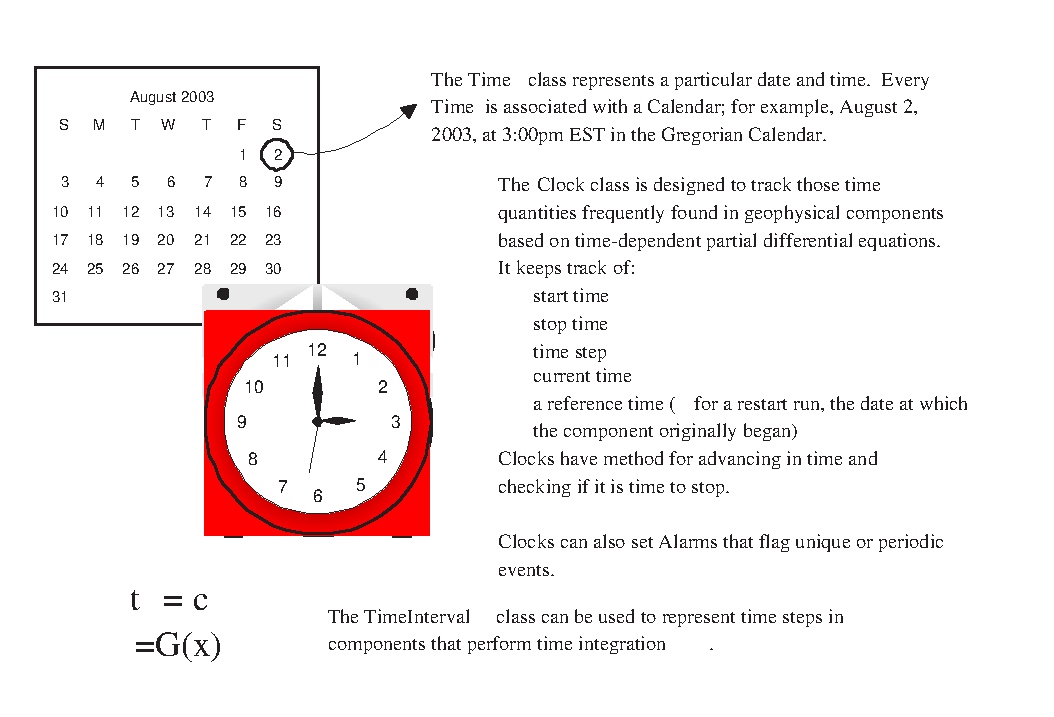
\includegraphics{TimeMgr_desc.eps}
%\end{center}

